\chapter{Background}\label{chap:background}
The ultimate goal of this thesis is to study a particular phenomenon (the MagnetoRotational Instability, MRI) in a particular regime (anisotropic viscosity) of plasma physics. In order to do so, it is helpful to be acquainted with the various plasma physics formalisms. This will be accomplished in Section~\ref{sec:plasmaphysics}. The numerical codes in use are explained in Section~\ref{sec:codes}, while the reason accretion is not trivial is outlined historically in Section~\ref{sec:early}. Equations are in Gaussian units unless otherwise specified. 

%------------------------------------------------------------------------%


\section{Plasma Physics} \label{sec:plasmaphysics}
Plasma physics applies to a wide range of subject areas, from magnetic-confinement fusion pursuits like the tokamak ITER~\cite{Janeschitz2001} and the stellarator Wendelstein 7-X~\cite{Grieger1993} to a variety of astrophysical situations, including the sun's corona and protoplanetary disks. The uniting theme across these different disciplines is the plasma: so what exactly is a plasma? \\
\\
A plasma is the so-called ``fourth state of matter'', coming after the gas phase in the increasing kinetic energy hierarchy solid-liquid-gas: that is, the inetic energy of a plasma particle is much greater than its potential energy. A plasma is made up of neutrals and the result of the neutrals' ionization: that is, ions and electrons. The basic physics of single-particle motion in electric and magnetic fields (for example, $\nabla B$ drift and $E\times B$ drift) apply to every single particle. Given the enormous quantity of particles, working analytically or simulating such a situation for each individual particle is near impossible. Indeed, this is why the kinetic theory is so complicated and requires particle-in-cell simulations that use codes such as PEGASUS (Section~\ref{sec:codes}). The task of this thesis is to make simulations feasible via (modified) fluid equations. 

\subsection{Characteristic Plasma Parameters}
One parameter that will be frequently discussed (since it determines the model that describes a plasma) is the mean free path $\lambda_{mfp}$ of a plasma particle, that is, how far it travels on average before it collides with another particle. This is related to the thermal velocity $v_T=\sqrt{2T/m}$ and collision frequency $\nu$ by
\begin{equation}
  \lambda_{mfp}=\frac{v_T}{\nu}=\frac1\nu\sqrt{\frac{2T}{m}}
\end{equation}
Notice that since the mass of an electron is so small compared to that of an ion (made up of protons and neutrons), the electron thermal velocity is much greater than the ion thermal velocity.\\
\\
The collision frequency $\nu$ depends on the temperature and density of a species as
\begin{equation}
  \nu\sim nT^{-3/2}
\end{equation}
Hence an increase in temperature leads to an increase in the mean free path of a particle because it decreases the collision frequency. In general, a higher collision rate simplifies calculations~\cite{Hazeltine2004}. This is because collisions push particles towards the Maxwell-Boltzmann (or Maxwellian) distribution of thermal equilibrium. Ideal MHD assumes a Maxwellian distribution. It is departures from this equilibrium that complicate calculations.\\
\\
Now we turn to defining magnetization is plasmas, which is an important definition in Braginskii MHD. The most important parameter is the easily-derivable thermal gyroradius: $\rho_s\equiv v_{T_s}/\Omega_s$ where $\Omega_s=q_sB/m_s$ (Gaussian units). A magnetized plasma is one for which the dimensionless parameter $\delta\equiv\rho/L$ goes to zero. In this case, particles will follow orbits that oscillate many times about magnetic field lines as their guiding center travels along the field lines. In ideal MHD, both $\lambda_{mfp}\ll L$ and $\delta\ll L$, whereas Braginskii MHD takes $\rho\ll\lambda_{mfp}\ll L$ and a collisionless plasma has $\lambda_{mfp}\gtrsim L$.\\
\\
As will be explained more later, the balance of magnetic pressure to gas pressure is also an important parameter. The plasma parameter, or $\beta$, as it is called, is given by:
\begin{equation}
  \beta=\frac{8\pi P}{B^2}
\end{equation}
where $P$ is the plasma pressure and $B$ is the magnetic field. $\beta$ is generally much larger in astrophysical systems (order of hundreds or thousands) than in magnetic-confinement fusion, where $\beta$ is usually around .01.\\
\\
Having established some basic properties of a plasma, we can now investigate some theories to model them, starting with kinetic theory.

%-------------------------------------------------------------------------------------%

\subsection{Vlasov Kinetic Theory} \label{ssec:vlasov}
Kinetic theory generalizes the brute-force method of applying Maxwell's equations (and the Lorentz Force Law) to many particles. The main result, known as the Vlasov equation, is:
\begin{align}
  \frac{\partial f_s(\vec x,\vec v,t)}{\partial t}+\vec u_k\frac{\partial f_s}{\partial x_k}+\frac qm (\vec E+\frac{\vec v}{c}\times\vec B)_k\frac{\partial f_s}{\partial v_k}=C[f_s] \label{eq:vlasov}
\end{align}
where $f_s$ is the phase-space density, or distribution function, which depends on the phase-space coordinates $\vec x$ and $\vec v$. In contrast, $\vec u_k$ is the velocity of particle $k$ with charge $q$ and mass $m$ in electric and magnetic fields $\vec E$ and $\vec B$. The left side depends only smoothly-varying terms, whereas the right is spiky, being the average of products of delta functions. The righthand side represents the interactions between individuals particles, and we can lump all these effects into the so-called ``collision operator'' $C[f]$. Entire graduate courses can be taught on the collision operator so we will not delve too much into it here.\\
\\
We define the distribution function to be normalized such that:
\begin{equation}
  \rho(\vec x,t)=\int d^3\vec v f(\vec x,\vec v, t)\label{eq:nnorm}
\end{equation}
where $\rho$ is the mass density and we have summed over species. Conservation laws emerge by taking different moments of the Vlasov equation and the collision operator. The $k$-th moment is defined as taking the integral $\int d^3v \vec v^k f_s$. Such moments are usually done in the frame moving with the bulk velocity of the fluid. Particle conservation, for example, arises from taking the zeroth-moment of the distribution function. \\
\\
A problem arises, however: every conservation law involves a higher moment of the distribution function. The evolution of density involves velocity, evolution of velocity involves the pressure tensor $\vec P$, evolution of the pressure involves the heat flux tensor $\vec Q$, and so on. This pattern of always involving higher moments of the distribution function does not simply disappear. Rather, it is a central problem of plasma physics known as the BBGKY hierarchy. It is various choices to ``close'' this loop of higher moments that defines different theories, including the standard ideal or ``single-fluid'' MHD. \\
\\
Methods to close the moment equations fall broadly into three categories: truncation, cases with special values for the distribution function or stress tensor, and asymptotic methods. The most straightforward solution is to simply truncate the hierarchy: just call the heat flux tensor $\vec Q=0$. This method can lead to useful intuition, but also means that the amount of error is not well-accounted for at all. There are also special cases such as having a Maxwellian distribution function (and thus assuming local thermal equilibrium) or assuming a cold plasma that eliminate the need for the fourth moment equation~\cite{Hazeltine2004}. The last closure method is that of asymptotics. This method generally assumes an ordering of certain parameters and expands about small values; which parameters are large or small depends on the exact type of asymptotic closure. This method is thereby more rigorous and the one that leads to ideal and Braginskii MHD, discussed below. \\
\\
The standard so-called ``MHD ordering'' assumes a magnetized plasma and takes $\delta\equiv\rho/L\ll1$. Assumptions from this point forward divide MHD into its different branches (for example, single-fluid ideal MHD and Braginskii MHD) and will be discussed in subsequent sections.

%----------------------------------------------------%

\subsection{Single-fluid MHD} \label{sec:idealMHD}
In single-fluid MHD, all species are treated as a single fluid. That is, to lowest-order they all have the same temperature and flow velocity and we average out the individual particles' positions and velocities. The important quantities are bulk variables, like the mean flow of the fluid, density, and pressure (one can already see how these variables might not make as much sense for an extremely diffuse plasma such as the weakly collisional ones described in Chapter~\ref{chap:introduction}).\\
\\
We consider MHD with the transport coefficients $\eta$ and $\nu$, the resistivity and shear viscosity, respectively. Ideal MHD can be obtained by setting these numbers to zero. The full set of equations is the moment equations combined with Maxwell's equations:
\begin{align}
  0&=\rho\frac{\partial\vec v}{\partial t}+(\rho\vec v\cdot\nabla)\vec v+\nabla P-\frac1{4\pi}(\nabla\times\vec B)\times\vec B-\nu\left(\nabla^2\vec v+\frac13\nabla(\nabla\cdot\vec v)\right)\label{eq:momentum}\\
  0&=\frac{\partial\rho}{\partial t}+\nabla\cdot(\rho\vec v)\label{eq:continuity}\\
  0&=\frac{\partial \vec B}{\partial t}-\nabla\times(\vec v\times\vec B-\eta\nabla\times\vec B)\label{eq:induction}\\
  0&=\frac{Dp}{Dt}+\frac53p\nabla\cdot\vec v
\end{align}
Here, the ``convective derivative'' $\frac{D}{Dt}=\frac{\partial}{\partial t}+\vec v\cdot\nabla$, where $\vec v$ is the center of mass motion of the fluid. This derivative accounts for both temporal and spatial variation as a fluid element moves along with the bulk motion of the rest of the fluid. The adiabatic index $\gamma$ depends on the equation of state. Isothermal evolution ($P=\rho c^2$, where $c$ is the speed of sound) takes $\gamma=1$. This thesis will consider adiabatic evolution with $\gamma=5/3$, that of a monatomic ideal gas.\\
\\
The moment equations are the first two equations, known respectively as the continuity and momentum equation, with Maxwell's equations slipped into the momentum equation and appearing as the induction equation (\ref{eq:induction}). This can be seen by considering Ohm's law: $\vec J=\sigma(\vec E+\frac1c\vec v\times\vec B)$, where $\sigma$ is the plasma conductivity. Combining with Ampere's law $\vec J=\frac{c}{4\pi}\nabla\times\vec B$ after neglecting the displacement currents since the fluid is nonrelativistic, we have $\vec E=\frac{c}{4\pi\sigma}\nabla\times\vec B-\frac1c\vec v\times\vec B$. Now using Faraday's law, we have $\frac1\sigma\nabla\times\vec J-\frac1c\nabla\times(\vec v\times\vec B)=-\frac1c\frac{\partial B}{\partial t}$, which leads to the induction equation after identifying $\eta=c^2/4\pi\sigma$. The other Maxwell's laws are contained in the assumption of quasi-neutrality $\sum_s n_sq_s=0$ (Gauss's law) and by imposing the initial condition $\nabla\cdot\vec B=0$, which will then remain true. \\
\\
We can use a vector identity to make the separation of the magnetic field energy into two components obvious: $(\nabla\times\vec B)\times\vec B=(\vec B\cdot\nabla)\vec B-(\nabla\vec B)\cdot\vec B=(\vec B\cdot\nabla)\vec B-\frac12\nabla B^2$ where $B^2=\vec B\cdot\vec B$. The magnetic pressure $\nabla B^2$ term tries to increase the spacing between magnetic field lines, making the parallel with normal pressure more obvious. The magnetic tension term $-\vec B\cdot\nabla\vec B$ term tries to unfurl curves in magnetic field lines. This term plays an important role in the mechanism of accretion discussed in Chapter~\ref{ssec:springs}.\\
\\
In ideal MHD, the magnetic field lines cannot diffuse since the plasma is perfectly conducting. This means that the field lines are effectively frozen into the plasma: the phenomenon is appropriately called ``flux-freezing'', or alternatively as Alfven's Theorem. Flux-freezing has important consequences for turbulence, since if a fluid particle is perturbed slightly, it will drag the magnetic field line with it. In non-ideal MHD, the field lines slip with respect to the rest of the plasma on the time scale of $\tau_R=\frac{\mu_0L^2}{\eta}$. This time scale will become important in Chapter~\ref{chap:compMRI}: for instance, if the dissipation time scale is shorter than characteristic time scales of the system (such as orbital time), then the magnetic field will decrease in energy, hindering the development of a magnetic dynamo. \\
\\
Non-ideal MHD carries with it a number of dimensionless numbers that characterize the relative importance of various quantities. For example, the Reynolds number is given by the ratio of inertial forces to viscous forces and can be written as $\mathrm{Re}=\frac{c_0}{H}\frac{H^2}{\nu}=\frac{c_0H}{\nu}$ where $c_0$ is the sound speed or other characteristic velocity in the fluid and $\nu$ is the viscosity. $H$ is the characteristic length scale, which here we take as the scale height of the disk. Thus the Reynolds number is the amount of dissipation on disk length scales in one sound crossing.\\
\\
The magnetic Reynolds number describes how important induction and advection of the magnetic field is compared to momentum advection of a fluid, while the ratio of the magnetic Reynolds number to the Reynolds number is called the magnetic Prandtl number:
\begin{equation}
  \mathrm{Pm}=\frac{\mathrm{Re_M}}{\mathrm{Re}}=\frac\nu\eta
\end{equation}
The magnetic Prandtl number accordingly measures how important viscous diffusion is relative to resistive diffusion. Higher Prandtl number means viscous dissipation is more important, and thus the velocity field is smoothed more than the magnetic field. In such situations we can expect more small-scale magnetic field eddies than velocity eddies. The hydrodynamic Prandtl number measures the importance of viscosity as compared to thermal diffusion and heat conduction rather than resistivity~\cite{Fromang2007b}. \\
\\
The importance of resistivity and viscosity has been explored in a number of papers~\cite{Fromang2007b,Lesur2007,Gammie1996} and plays an important role in the physics of accretion, as will be discussed in Chapter~\ref{chap:compMRI}.\\
\\
Since the point of this thesis is that MHD is not valid for certain kinds of plasmas, let us now examine the assumptions that went into these equations. We first assume that pressure is isotropic, which means the heat flux tensor disappears. Since we are here considering magnetized plasmas, we also take $\delta=\rho/L\to0$. Quasi-neutrality is a good simplification since plasmas are usually overall neutral in nature. Dropping the displacement current in Ampere's law is also fine, since as mentioned earlier, the characteristic velocity of particles in our system is the thermal velocity. Note that it is possible to include general relativity in these calculations; however, as mentioned in the introduction, this thesis is concerned with the limit in which general relativity is excessive.\\
\\
Lifting the requirement that pressure be isotropic and introducing a new ordering of scales leads to Braginskii MHD, described in the following section.

%-----------------------------------------------------------%

\subsection{Braginskii MHD} \label{ssec:bragMHD}
Braginskii MHD uses the assumptions that the time between collisions, while not zero, is much larger than typical time scales. Equivalently, the collisional frequency is much greater than other characteristic frequencies of the system. The appropriate limits are:
\begin{equation}
  \rho\ll\lambda_{mfp}\ll L \label{eq:bragord}
\end{equation}
Note that weakly collisional systems have mean free paths comparable to or larger than the length scales of the system: we therefore have no apparent reason to trust Braginskii MHD in a weakly collisional regime! Such is the motivation of this thesis: we shall investigate whether we can actually accomplish a meaningful approximation.\\
\\
Because the magnetic field is so strong and the gyromagnetic radius is so small compared to the mean free path, we can write the motion of particles as a sum of the guiding center motion and the gyrotropic motions about the field lines. This leads to an anisotropic pressure tensor
\begin{equation}
  \vec{p}=
  \begin{pmatrix}
  p_\parallel & 0 & 0\\
  0 & p_\perp & 0\\
  0 & 0 & p_\perp
  \end{pmatrix}
\end{equation}
if $\hat x=\hat b$ is along the magnetic field. Note that the isotropic pressure $p=\frac23p_\perp+\frac13p_\parallel$ and hence $p_\perp=p+\frac13(p_\perp-p_\parallel)$ and $p_\parallel=p-\frac23(p_\perp-p_\parallel)$. \\
\\
Rigorously what follows is an expansion of the distribution function about a Maxwellian (see, e.g.,~\cite{Negulescu2016}). However, we take a more intuitive approach here and simply argue for adding collisional terms to the evolution equations for the pressures, which arise from conservation of adiabatic invariants.\\
\\
Adiabatic invariants are quantities that are ``conserved'' in the sense that they stay the same when changes in a system happen slowly enough. The two that we consider here are the magnetic moment $\mu$ and the mirror constant $J$:
\begin{align*}
  \mu&=\frac12m\frac{w_\perp^2}{B} &  J&\equiv m\oint w_\parallel dl
\end{align*}
These are conserved as long as $\big|\frac{D\ln B}{Dt}\big|\ll\Omega$ and $\big|\frac{D\ln B}{Dt}\big|\ll\omega_b$ where $\omega_b$ is the bounce frequency associated with the magnetic mirror under consideration. Following~\citet{KunzBraginskii}, we see how these invariants relate the anisotropic pressure and the magnetic field:
\begin{align}
  \langle\mu\rangle&\sim\frac{p_\perp}{Bn}=\frac{T_\perp}{B} &  \langle J^2\rangle&\sim\frac{mB^2}{n^3}p_\parallel=\frac{B^2}{n^2}T_\parallel m\label{eq:javg}
\end{align}
with $T_{\parallel,\perp}=p_{\parallel,\perp}/n$, where $n$ is the number density instead of the mass density $\rho$ for ease of telling $p$ and $\rho$ apart. An increase in the magnetic field strength will lead to an increase in perpendicular pressure, which will increase the pressure anisotropy. Combining these equations, we can come up with an equation for the evolution of the pressure anisotropy. We know that collisions push the distribution function back to a Maxwellian; therefore, we keep the pressure anisotropy small, moderated by the small parameter $\nu_{coll}$:
\begin{align*}
  \frac{Dp_\perp}{Dt}&=p_\perp\left(\frac{D\ln Bn}{Dt}\right)-\nu_{coll}(p_\perp-p)\\
  \frac{Dp_\parallel}{Dt}&=p_\parallel\left(\frac{D\ln B^{-2}n^3}{Dt}\right)-\nu_{coll}(p_\parallel-p)
\end{align*}
Subtracting these and setting the derivative of the pressure anisotropy to zero as prescribed by the Braginskii approximation, we obtain the Braginskii closure:
\begin{align}
  p_\perp-p_\parallel&=\frac{3p}{\nu_{coll}}\frac{D}{Dt}\ln\frac{B}{n^{2/3}}=\frac{3p}{\nu_{coll}}\left(\hat b\hat b-\frac{\vec{\mathbb{I}}}{3}\right):\nabla\vec u \label{eq:bragclos}
\end{align}
The right hand side, the adiabatic invariance, produces the pressure anisotropy on the left hand side. One might conclude that, without collisions, anisotropy is produced uncontrollably. This is however not true because the adiabatic invariants are no longer conserved once certain thresholds are reached~\cite{Sharma2006}. \\
\\
The collisionless version of this closure, known as the double-adiabatic or Chew-Goldberger-Low (CGL) closure, was originally developed for fusion devices. We shall use the Braginskii formalism because of the many problems accrued by the CGL closure in astrophysical situations~\cite{Sharma2006}.\\
\\
We can now write the MHD equations in terms of this closure. Some work yields:\\
\begin{align*}
  \frac{D\ln n}{Dt}&=-\nabla\cdot\vec u\\
  \frac{D\ln B}{Dt}&=(\hat b\hat b-\mathbb{\vec I}):\nabla\vec u\\
  \frac32p\frac{D\ln pn^{-5/3}}{Dt}&=\frac{3p}{\nu_{coll}}\left[\left(\hat b\hat b-\frac{\vec{\mathbb{I}}}3\right):\nabla\vec u\right]^2\\
  mn\frac{D\vec u}{Dt}&=-\nabla\left(p_\perp+\frac{B^2}{8\pi}\right)+\frac{\vec B\cdot\nabla\vec B}{4\pi}+\nabla\cdot\left[\frac{3p}{\nu_{coll}}\left(\hat b\hat b-\frac13\vec{\mathbb{I}}\right)^2:\nabla\vec u\right]
\end{align*}
The right hand side of the entropy equation in the form of $|\nabla\vec u|^2$ represents viscous heating. Clearly, the viscous heating is anisotropic. But what does this mean? Examining the right hand side more closely, we see that the vector $\hat b\hat b-\vec{\mathbb{I}}/3$ selects out the direction perpendicular to the magnetic field. Therefore, velocity gradients perpendicular to the magnetic field are wiped out by the dot product, whereas velocity gradients parallel to the magnetic field survive to be viscously damped. The same holds true for the momentum equation. We are led to conclude that there are no collisions across magnetic field lines, while there are collisions along magnetic field lines, leading to viscous momentum transport along field lines. Braginskii's ordering~\ref{eq:bragord} forbids particles from moving across the field lines more than a distance of a mean free path. The situation is illustrated in Figure~\ref{fig:bragviscosity}.\\
\\
Extending this closure to the heat flux moment equation leads to anisotropic heat flux along field lines and several instabilities (including the MagnetoThermal Instability (MTI) and Heat-flux-driven Buoyancy Instability (HBI)), which have been studied both analytically and numerically for applications to the ICM and winds in hot accretion flows~\cite{KunzBraginskii,Balbus2000,Balbus2001,Kunz2011,Parrish2007,Parrish2005,Johnson2007,Bu2016,Quataert2008,Parrish2008a}.
%
\begin{figure}[h]
  \begin{center}  
    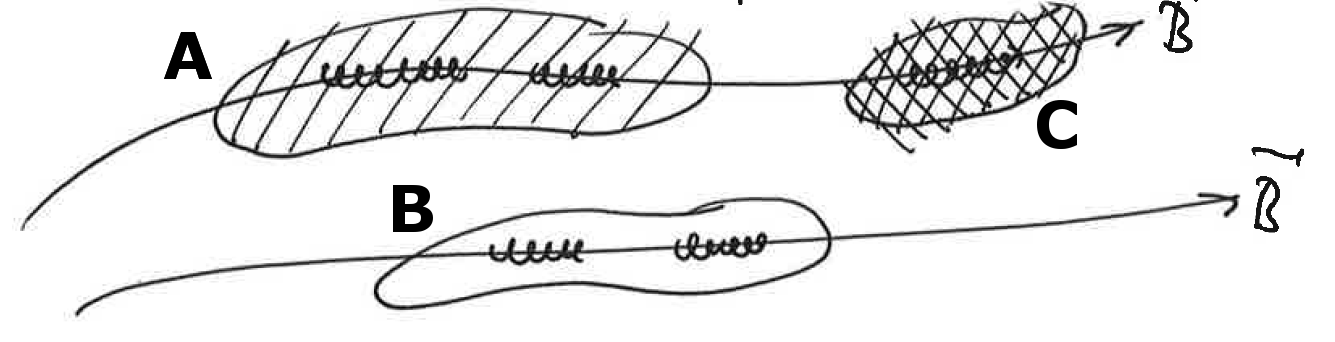
\includegraphics[width=\textwidth, angle=0.]{img/paralleltransport.png}
  \end{center}
  \caption{Transport of momentum along magnetic field lines $\vec B$. Packets of particles are shown in the blobs labelled A, B, and C. Particle paths of each packet in Larmor motion about the field lines is also shown. Packet A can interact and collide with Packet C, but Packet B cannot interact with either Packet A or C because they lie on different field lines. From~\citet{KunzBraginskii}.}
  \label{fig:bragviscosity}
\end{figure}

\subsection{Kinetic effects closure}\label{ssec:kinclosure}
There are several approaches to modifying the fluid equations to capture kinetic effects.~\citet{Sharma2003} has studied the transition from collisionless theory to MHD theory and found that the key difference is anisotropic collisions. This same anisotropy was present in the Braginskii MHD equations in the previous section. Braginskii MHD thus seems like an appropriate starting point off of which we can build in additional modifications to attempt to replicate kinetic effects.\\
\\
Studies of kinetic theory over the years has shown that additional ``parasitic'' instabilities limit the growth of the pressure anisotropy~\cite{SharmaThesis, Kunz2016}. The three most important instabilities are the firehose, mirror, and ion cyclotron instabilities. The third sets a looser limit than the mirror instability and thus will not be included~\cite{Sharma2006,Riquelme2015}. \\
\\
The thresholds for instability to the firehose and mirror instability, are respectively~\cite{Kunz2016,Kunz2014,Schekochihin2008,Sharma2006}:
\begin{align}
  \frac{p_\perp}{p_\parallel}-1+\frac2{\beta_\parallel}&>0 & \frac{p_\perp}{p_\parallel}-1&<\frac{1}{\beta_\perp} \label{eq:mirrorthresh}
\end{align}
These instabilities are not due to collisions since the plasma is collisionless. They are rather Alfven waves destabilized by the pressure anisotropy~\cite{Sharma2006}. These waves tangle up the magnetic field of the plasma on the scale of the Larmor radius, which throws particles off of their trajectory. We can therefore model these instabilities as having an effective collision rate and thus a resistivity and viscosity~\cite{Schekochihin2008}.\\
\\
In light of the thresholds above, we manually cap the pressure anisotropy over the course of our simulations in Chapter~\ref{chap:kinbrag}. The hope is that such an anisotropy maximum will sufficiently capture the kinetic instabilities in a fluid closure, as discussed in Chapter~\ref{chap:kinbrag}.

%------------------------------------------------------------------%

\section{Codes: Athena4.2 and Pegasus} \label{sec:codes}
The systems under consideration in this thesis are extremely complicated and thus require the use of simulations to model on large time or length scales. Two codes are used for this purpose: one, an MHD solver, the other, a hybrid-kinetic particle-in-cell (PIC) code.\\
\\
The code in use in Chapters~\ref{chap:compMRI} and~\ref{chap:kinbrag} to simulate MHD systems is Athena4.2 (henceforth referred to as Athena). Athena, a response to the older code ZEUS, uses a higher-order Godunov scheme for flexibility and the constrained transport technique to ensure a divergence-free magnetic field. It is a highly-modularized grid-based code with additions such as adaptive mesh refinement (AMR) capabilities, special relativity, and dust~\cite{Stone2008,Stone2009}. The shearing box approximation (as explained in Section~\ref{ssec:shearingbox}) has also been implemented~\cite{Stone2010}. A new version of Athena, Athena++, more easily integrates general relativity and allows for better Riemannien solvers~\cite{White2016Thesis,White2016}.\\
\\
For collisionless and weakly collisional plasmas, the distribution function itself must be evolved. Such evolution is accomplished with a so-called ``particle-in-cell'' or PIC code. Because a fully-kinetic code usually requires compromising assumptions such as reduced speed of light or a smaller ion-to-electron mass ratio, hybrid-kinetic codes such as PEGASUS, the one used in~\citetalias{Kunz2016} that this thesis compares its results to in Chapter~\ref{chap:kinbrag}, are perhaps more useful. PEGASUS itself treats electrons as a massless fluid, while ions are treated kinetically. This assumption is valid since ions are much hotter than the efficiently-radiating electrons~\cite{Das2013}. PEGASUS is a second-order accurate code that uses a three-stage predictor-predictor-corrector algorithm for integration. It also uses the constrained transport method as Athena does to enforce a divergence-less magnetic field and implements the shearing box method~\cite{Kunz2014}. \\
\\
Codes were run on Princeton's Della and Perseus clusters using Tigress for intermediate data storage.

%---------------------------------------------------------------------%

\section{Early Problems in Accretion}\label{sec:early}
The above sections have addressed the fundamental plasma physics behind radiatively-inefficient accretion flows and how they are implemented numerically. But how does accretion actually work on a fundamental level? \\
\\
Accretion is the outward transport of angular momentum, which means that particles that lose angular momentum drop closer to the central accreting object (in the case of this thesis, a black hole) in accordance with differential rotation. It seems natural to explain this slowing down via friction; in an accretion disk, the matter at different radii are not moving at the same velocity (i.e. there is a shear) and hence one might think that there is a sort of coefficient of kinetic friction between particles that slows down their movement and causes them to accrete. The idea that this ``molecular'' or ``shear'' viscosity could explain accretion rates is tempting, but in reality is not supported by simulations or observations.\\
\\
Early simulations and observations showed accretion rates on the order of $10^{15}cm^2/s$; however, the standard values of molecular viscosity are in the tens of $cm^2/s$, somewhere around 14 orders of magnitude too small~\cite{Spruit2009}. This fantastic difference between theory and simulations resulted in several new ideas for explaining the transport of angular momentum and led to the formulation of one of the most well-known models for thin disks---the $\alpha$-disk.\\
\\
The seminal paper of ~\citet{SS1973} explores accretion disks in the context of a binary star system. It essentially characterizes ignorance in the accretion rate via the parameter $\alpha$, defining the tangential stress $w_{r\phi}=\alpha\rho v_s^2$, where $v_s$ is the sound speed such that $\rho v_s^2/2$ is the disk matter's thermal energy density, although definitions vary to order unity across sources~\cite{SS1973}. This formulation provides a parameter that is easy to tweak in numerical simulations and is still in use today~\cite{Penna2013}. \\
\\
Despite its intuitive usefulness, the $\alpha$ prescription offers no mechanism for the transport of angular momentum. It was proposed that, while pure molecular viscosity could not explain the observed accretion rates, an ``effective'' viscosity due to eddy interaction could do the job~\cite{BH1998}. In other words, turbulence would generate eddies whose interactions would manifest similar to a viscosity. The problem became to find the source of the turbulence that would lead to outward angular momentum transport. Supposing that an effective viscosity generated by turbulence can explain observed and simulated accretion rates, the question becomes: what causes this turbulence? \\
\\
Some, influenced by laboratory fluid mechanics, believed that the sheer property of having a high Reynolds number (huge in astrophysical flows due to the large length scales involved) satisfactorily accounted for the needed turbulence. This allows for free energy to be extracted from the shear flow. However, Keplerian flows are stable against perturbations (i.e. experience no turbulence) where shear flows are not (Rayleigh's criterion for stability is that the specific angular momentum increases radially outward). The difference is due to epicycles in Keplerian flows, which sink the energy that would otherwise devolve into prominent disturbances. A high Reynolds number is not enough to explain the necessary turbulence.\\
\\
It was long thought that hydrodynamic convective instabilities could lead to turbulence in accretion disks~\cite{Paczynski1978,Stone1999}. Other possibilities include non-local effects such as waves and shocks created by tidal forces. These effects can produce accretion at rates up to $\alpha=.01$, but only in hot disks~\cite{Spruit2009}. Global disk winds, of the type suggested by~\citet{Blandford1977}, could also transport angular momentum. These magnetically-driven winds could theoretically sweep matter around in such a way as to account for the high accretion rates without a viscosity while also helping account for AGN jets~\cite{Koenigl1989}; however, the presence of these winds in all accretion disks is debated. A more universal and fundamental explanation seems more likely.\\
\\
Magnetic fields were thought to serve an amplifying role in turbulence transport. That is, with pre-existing turbulence, magnetic fields would tangle and speed along the transportation of magnetic fields~\cite{SS1973}. It was thought that the magnetic pressure and pressure due to turbulence were distinct, and that magnetic pressure would be insignificant in disk situations, or would require large magnetic fields on the order of $10^7-10^8$~G to balance the gravitational pressure of infalling gas~\cite{BH1998}. The magnetic field was mainly considered to be important due to consequences of cyclotron radiation as a cooling mechanism~\cite{Shapiro1973}. In 1991, Balbus and Hawley~\cite{BH1991a,BH1991b,BH1991c} closed the conceptual circle by showing that turbulence resulted directly from a weak magnetic field. Pre-existing turbulence was not needed; the entire sequence of generating turbulence and transporting turbulence and angular momentum could be derived as a result of a linear instability in the MHD equations (see Section~\ref{sec:localideal}). Numerous numerical simulations have since confirmed the important role of magnetic fields in accretion processes. The next chapter will explore this linear instability in the context of numerical simulations.

\section{Past Work on Anisotropic Viscosity}
Anisotropic viscosity has been studied in numerous previous works both analytically and numerically. The linear regime of Braginskii MHD has been studied to find the dispersion relation, growth rates, and fastest-growing modes after some ``straightforward but somewhat tedious algebra'' which will not be replicated here~\cite{Balbus2004,Islam2005}. Stability of the disk has also been investigated~\cite{Quataert2015}. The nonlinear regime of turbulence, of interest in this thesis, must be studied numerically and has been done so in the context of the magnetothermal instability~\cite{Bu2011}.\\
\\
The idea of using pressure anisotropy limiters comes from studies showing that the firehose and mirror instabilities destroy anisotropy even when finite Larmor radius effects are taken into account~\cite{Hellinger2000,Hellinger2007}.~\citetalias{Sharma2006} has implemented these limiters already; however, that paper uses a different formalism, namely, kinetic-MHD, to solve for the evolution of the magnetic field. It also calculates viscosity at every step, which is more computationally intensive than just setting the viscosity to have one value (the approach taken in this thesis). However,~\citetalias{Sharma2006} and~\citetalias{Kunz2016} both use $\beta=400$, which is what this thesis also uses for ease of comparison with both the kinetic-MHD regime (although other differences such a net-flux magnetic field prevent this comparison from being exactly parallel) and the fully-kinetic regime. \\
\\
This thesis investigates the ability of an old theory (Braginskii MHD) with the pre-existing idea of pressure anisotropy limiters to approximate the new results of a more complex theory. 



